\documentclass{beamer}
\usepackage{etex}
\usetheme{Antibes}
\usepackage{amssymb,amsmath,amsthm}
\usepackage{graphicx}
\usepackage{caption}
\usepackage{subfig}
\newcommand{\bn}{\begin{enumerate}[i)]}
\newcommand{\en}{\end{enumerate}}
\newcommand{\im}{\item}
\newcommand{\CPT}[1]{\large{\textbf{CHAPTER #1}}}
\newcommand{\ir}[1]{\textbf{Remark #1}}
\newcommand{\ith}[1]{\textbf{Theorem #1}}
\newcommand{\idf}[1]{\textbf{Definition #1}}
\newcommand{\iex}[1]{\textbf{Example #1}}

%\definecolor{cardinal}{rgb}{0.77, 0.12, 0.23}
%\usecolortheme[named=cardinal]{structure}
%\setbeamercolor{block title}{bg=cardinal,fg=black}
 \usepackage{tikz}
 \usetikzlibrary{patterns,snakes,plotmarks}
 \usepackage{multirow}
% \usetikzlibrary{shadows}
\usepackage{epstopdf}
\usepackage{nicefrac}
\usepackage{lmodern}
\usepackage{pgfplots}
\usepackage{qtree}
\newcommand*{\Scale}[2][4]{\scalebox{#1}{\ensuremath{#2}}}%
\DeclareCaptionLabelSeparator{horse}{:\,\,} % change according to your needs
\captionsetup{
  labelsep = horse,
  figureposition = bottom % used to get the correct vertical space between the figure and the caption
}
\setbeamertemplate{caption}[numbered]
\setbeamertemplate{items}[circle]
\setbeamertemplate{enumerate items}[square]
\theoremstyle{definition}
\newtheorem*{exs}{Examples}
\newtheorem{ex}{Example}
\newtheorem*{exc}{Exercise}
%\usepackage{booktabs}
\setlength{\parindent}{0pt}
%\setbeameroption{show notes}
 \setbeamerfont{note page}{size=\tiny}
%\setbeamertemplate{note page}[plain]
%\setbeameroption{show only notes}
\title{Math 629 - Survival Analysis \\ Chapter 2}
\author{Drew Lazar}
\institute{Ball State University}
\date{\today}

\begin{document}
\begin{frame}
    \titlepage
\end{frame}
\section{Chapter 2}

\begin{frame}
\frametitle{Constructing Kaplan-Meirer Curves}
Consider the following data (from chapter 1) of times to remission of leukemia patients:
\begin{block}{Remission Data }
\begin{table}
\begin{center}
\begin{tabular}{l l}
Group 1 (n=21) treatment & Group 2 (n=22) placebo \\
 6, 6, 6, 7, 10, 13, 16, 22, 23, & 1, 1, 2, 2, 3, 4, 4, 5, 5,  \\
 6+, 9+, 10+, 11+, 17+, 19+, & 8, 8, 8, 8, 11, 11, 12, 12, \\
   20+, 25+, 32+, 32+, 34+, 35+ & 15, 17, 22, 23
\end{tabular}
\end{center}
\end{table}
Note: + denotes censored
\end{block}
\end{frame}

\begin{frame}
\frametitle{Constructing Kaplan-Meirer Curves (cont'd)}
\begin{block}{Remission Data (another way)}
\begin{columns}
    \begin{column}{0.48\textwidth}
        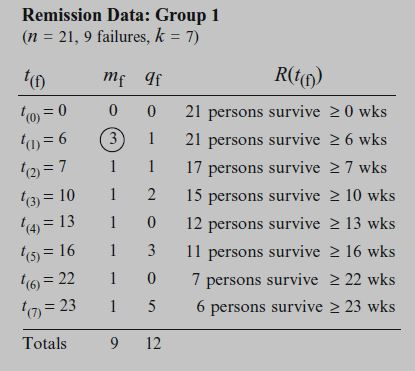
\includegraphics[width =\textwidth, height=6cm]{Ch1-leuk_data_a1.JPG}
    \end{column}
    \hspace{-10pt}
    \begin{column}{0.48\textwidth}
         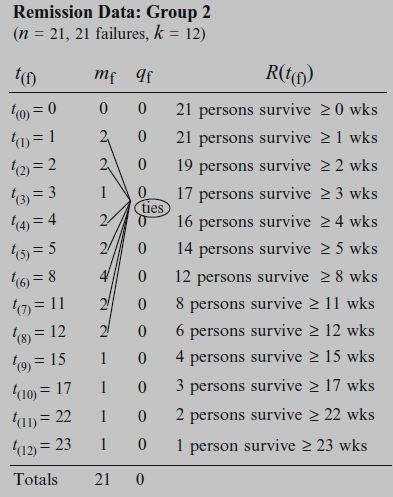
\includegraphics[width =\textwidth, height=6cm]{Ch1-leuk_data_b1.JPG}
    \end{column}
\end{columns}
\end{block}
\end{frame}


\begin{frame}
\frametitle{Constructing Kaplan-Meirer Curves (cont'd)}
\begin{block}{Kaplan-Meirer Estimates for Group 2}
\begin{columns}
    \begin{column}{0.48\textwidth}
        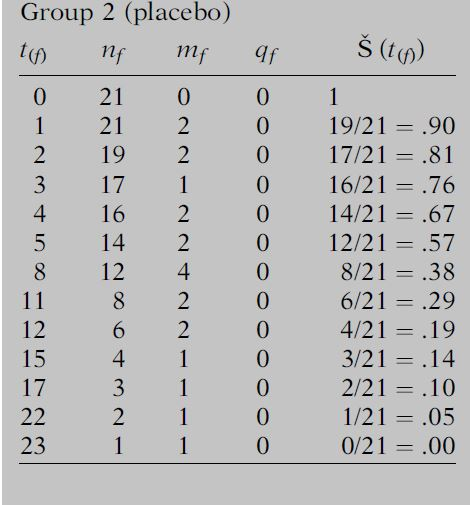
\includegraphics[width =\textwidth, height=5.5cm]{Ch2_KMGP2.JPG}
    \end{column}
    \hspace{-10pt}
    \begin{column}{0.48\textwidth}
         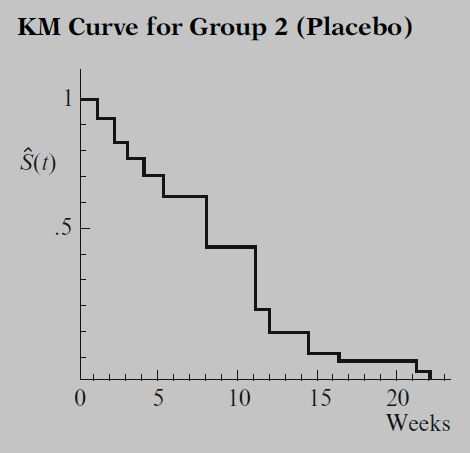
\includegraphics[width =\textwidth, height=5.5cm]{Ch2_KMCGP2.JPG}
    \end{column}
\end{columns}
\end{block}
\end{frame}

\begin{frame}
\frametitle{Constructing Kaplan-Meirer Curves (cont'd)}
\begin{block}{Problem 2.1 - Kaplan-Meirer Estimates for Group 1}
         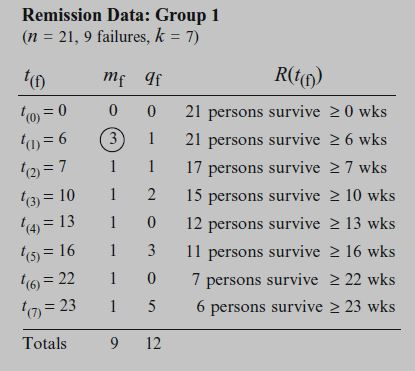
\includegraphics[width =\textwidth, height=5.5cm]{Ch1-leuk_data_a1.JPG}
\end{block}
Find the Kaplan-Meirer Estimates for Group 1 and plot the Kaplan-Meirer Curves for groups 1 and 2.
\end{frame}

\begin{frame}
\frametitle{Constructing Kaplan-Meirer Curves (cont'd)}
\begin{block}{Kaplan-Meirer Curves for Groups 1 and 2}
         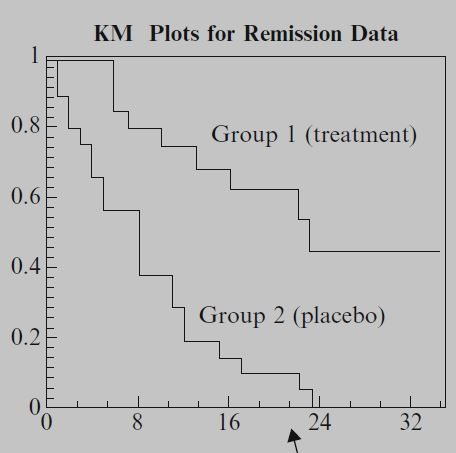
\includegraphics[width =\textwidth, height=5.5cm]{Ch2_KM_GR12.JPG}
\end{block}
\end{frame}

\begin{frame}
\frametitle{Constructing Kaplan-Meirer Curves (cont'd)}
\begin{block}{Problem 2.2 - Kaplan-Meirer Estimates in R}
\begin{enumerate}
\item Find the KM Estimates for the entire remission data set in R
\item Plot the KM curve for the entire remission data set in R
\item Find the KM Estimates for group 1 and group 2 in R
\item For groups 1 and 2 and plot the KM Curves for Groups 1 and 2 in R
\end{enumerate}
\end{block}
\end{frame}

\begin{frame}
\frametitle{Log-Rank Tests for Survival Experiences}
\begin{block}{Log-Rank Tests for two groups}
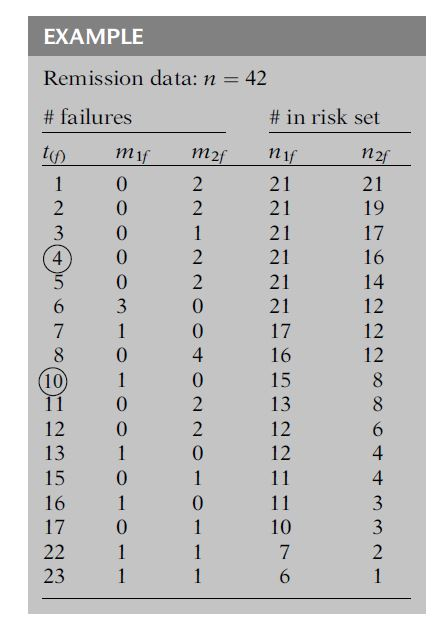
\includegraphics[width =\textwidth, height=5.5cm]{CH2_LogRank.JPG}
\end{block}
\end{frame}

\begin{frame}
\frametitle{Log-Rank Tests for Survival Experiences (cont'd)}
\begin{block}{Log-Rank test for two groups}
We can test whether the null hypothesis, $H_0$, that the survival experiences for these two groups is the same as follows.
\begin{enumerate}
\item Find the \textbf{expected cell counts}.
\begin{align*}
e_{1f} & = \left(\frac{n_{1f}}{n_{1f} + n_{2f}}\right)(m_{1f} + m_{2f}) \\
e_{2f} & = \left(\frac{n_{2f}}{n_{1f} + n_{2f}}\right)(m_{1f} + m_{2f})
\end{align*}
\end{enumerate}
\end{block}
\end{frame}

\begin{frame}
\frametitle{Log-Rank Tests for Survival Experiences (cont'd)}
\begin{block}{Log-Rank test for two groups (cont'd)}

\begin{enumerate}
 \setcounter{enumi}{1}
\item Find the total number of observed minus expected failures
\[
O_i - E_i = \sum_{f=1}^k (m_{if} - e_{if}), \, i=1,2
\]
Where $k$ is total number of events. \\
We must have $O_1 - E_1 = -(O_2- E_2)$.
\end{enumerate}
\end{block}
\end{frame}

\begin{frame}
\frametitle{Log-Rank Tests for Survival Experiences (cont'd)}
\begin{block}{Log-Rank test for two groups (cont'd)}
 \begin{enumerate}
  \setcounter{enumi}{2}
\item Form the log rank statistic
\[
LRS = \frac{(O_i - E_i)^2}{\text{Var}(O_i-E_i)} \text{ for } i=1 \text{ or } i=2
\]
or approximate LRS
\[
LRS = \sum_i^{2} \frac{(O_i - E_i)^2}{E_i}
\]
\item Reject $H_0$ iff $\text{LRS} > \chi^2_{\alpha,1}$ where $\alpha$ is the significance of test or
\[
\text{p-value} = P(X>LRS), \,  X \sim \chi^2_1 \text{ reject iff p-value} \le \alpha.
\]
\end{enumerate}
\end{block}
\end{frame}

\begin{frame}
\frametitle{Log-Rank Tests for Survival Experiences (cont'd)}
\begin{block}{Log-Rank test for two groups (cont'd) - Remission Data}
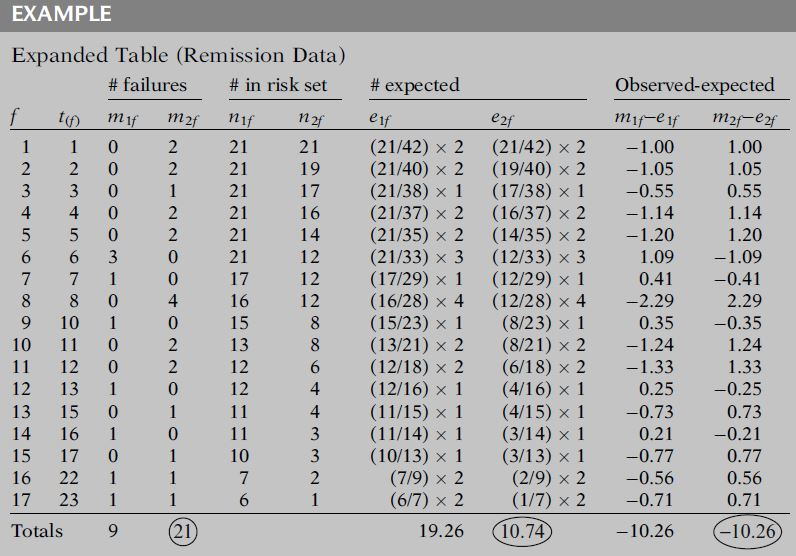
\includegraphics[width =\textwidth, height=5.5cm]{CH2_ComputeLR}
\end{block}
\end{frame}


\begin{frame}
\frametitle{Log-Rank Tests for Survival Experiences (cont'd)}
\begin{block}{Log-Rank test for $G>2$ groups}
The null hypothesis, $H_0$, is that the survival experiences for \textit{all} groups is the same.
\begin{enumerate}
\item Find the \textbf{expected cell counts}.
\begin{align*}
e_{if} & = \left(\frac{n_{if}}{n_{f}}\right)(m_{f}) \\
n_{f} & = \sum_{i=1}^G n_{if}, \, m_f =  \sum_{i=1}^G m_{if}\\
\end{align*}
where $n_{if}=$\# at risk at $t_f$ for group $i$, \, $m_{if}=$\# of failures at $t_f$ for group $i$.
\end{enumerate}
\end{block}
\end{frame}

\begin{frame}
\frametitle{Log-Rank Tests for Survival Experiences (cont'd)}
\begin{block}{Log-Rank test for $G>2$ groups}
\begin{enumerate}
 \setcounter{enumi}{1}
\item Find the total number of observed minus expected failures
\[
O_i - E_i = \sum_{f=1}^k (m_{if} - e_{if}), \, i=1,2, \ldots, G.
\]
where $k$ is total number of events.
\item Find approximate log-rank statistic
\[
LRS = \sum_i^{\text{\# groups}} \frac{(O_i - E_i)^2}{E_i}
\]
Exact LRS is given in Chapter 2 appendix.
\end{enumerate}
\end{block}
\end{frame}

\begin{frame}
\frametitle{Log-Rank Tests for Survival Experiences (cont'd)}
\begin{block}{Log-Rank test for $G>2$ groups}
\begin{enumerate}
\setcounter{enumi}{3}
\item Reject $H_0$ iff $\text{LRS} > \chi^2_{\alpha,G-1}$ where $\alpha$ is significance of test or
\[
\text{p-value} = P(X>LRS), \,  X \sim \chi^2_{G-1} \text{ reject iff p-value} \le \alpha.
\]
\end{enumerate}
\end{block}
\begin{block}{Vets data set}
Vets.dat reports on survival times in days for 137 patients from the Veteran’s Administration Lung Cancer Trial:
\begin{center}
\includegraphics[width =4.5cm, height=2.5cm]{CH2_Vets}
\end{center}
\end{block}
\end{frame}
\begin{frame}
\frametitle{Log-Rank Tests for Survival Experiences (cont'd)}
\begin{block}{Problem 2.3 - Log-Rank Tests in R}
\begin{enumerate}
\item In R conduct a Log-Rank test for the two groups in the Remission Data. What conclusion do you reach?
\item In R partition the Vets.dat data set into three groups by Performance Status: Group 1: 0-59, Group 2: 60-74 and Group 3: 75-100. Create and plot KM estimates for these three groups and conduct an overall log-rank test to test if the survival experiences are the same. What conclusion do you reach?
\end{enumerate}
\end{block}
\end{frame}
\begin{frame}
\frametitle{Variations and Extensions of the Log-Rank Test}
\begin{block}{Alternative Log-Rank Tests}
The Wilcoxon, Tarone-Ware, Peto and Flemington-Harrington tests work by weighting observed - expected numbers of events. That is, they weight terms in the log rank test
\[
O_i - E_i = \sum_f (m_{if}-e_{if}) \text{ to get } \sum_f w(t_{(f)})(m_{if}-e_{if})
\]
and use test statistic (below for $G=2$ groups)
\[
\frac{\left(\sum_f w(t_{(f)}) (m_{if}-e_{if})\right)^2}{Var\left(\sum_f w(t_{(f)})(m_{if}-e_{if})\right)}
\]
\end{block}
\end{frame}

\begin{frame}
\frametitle{Variations and Extensions of the Log-Rank Test (cont'd)}
\begin{block}{Alternative Log-Rank Tests (cont'd)}
We look at the Flemington-Harrington test. This test uses weights
\[ w(t_{(f)}) = (\hat{S}(t_{(f-1)}))^p (1-\hat{S}(t_{(f-1)}))^q \text{ with } p,q \ge 0.
\]

\begin{itemize}
\item If $p=q=0$ then we recover the log rank test.
\item If $q=0, p>0$ as $\hat{S}(t_{(f-1)})^p $ is a decreasing (non-increasing) function of $f$, earlier times are going to weigh more heavily in determining differences than later times.
\item If $p=0, q>0$ as $[1-\hat{S}(t_{(f-1)})]^q $ is an increasing (non-decreasing) function of $f$, earlier times are going to weigh less heavily in determining differences than later times.
\item Given $q=0$ how differences are weighed can be determined by examining the function $x^p$ for various $p>0$.
\end{itemize}
\end{block}
\end{frame}

\begin{frame}
\frametitle{Variations and Extensions of the Log-Rank Test (cont'd)}
\begin{block}{Alternative Log-Rank Tests (cont'd)}
Assume in the Flemington-Harrington test $q=0$. For $p=3$ the importance of earlier times falls off quickly and then flattens. For $p=0.15$ the importance decreases slowly then falls off quickly at the end.
\begin{center}
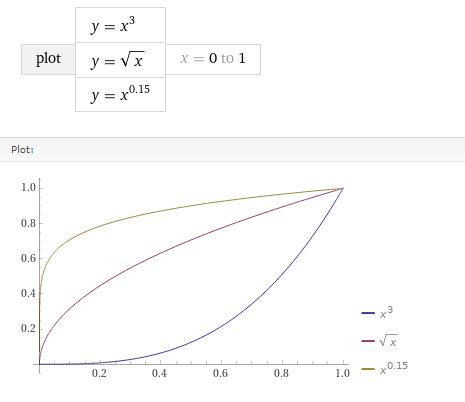
\includegraphics[width =4.5cm, height=3.5cm]{Ch2_Flemharringtonplot.JPG}
\end{center}
\end{block}
\end{frame}

\begin{frame}
\frametitle{Variations and Extensions of the Log-Rank Test (cont'd)}
\begin{block}{Problem 2.4 - Alternative Log-Rank Tests (cont'd)}
Conduct the Flemington-Harrington Test in R with $q=0$ and $p=0, 0.15, 0.5$ and 3 to compare the Placebo vs. Treatment groups in the remission data. Considering the Kaplan-Meirer estimates below, what should happen to the Chi-Square statistic as $p$ increases?
\end{block}
\begin{center}
         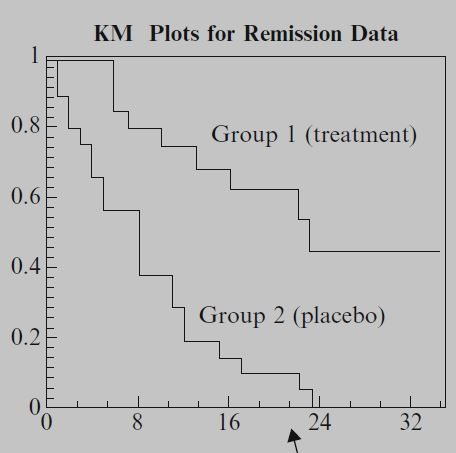
\includegraphics[width =5.0cm, height=4.0cm]{Ch2_KM_GR12.JPG}
\end{center}
\end{frame}

\begin{frame}
\frametitle{Variations and Extensions of the Log-Rank Test (cont'd)}
\begin{block}{The stratified log rank test}
If there is confounding, then the log rank test with respect to the exposure variable can be misleading. Instead, we can stratify on the confounding variable, compute observed and expected number of events at each time across strata.
\[
O_i-E_i = \sum_s \sum_f (m_{ifs} - e_{ifs})
\]
where $i=$ group, $f=$failure time, $s=$stratum.
Then we compute (approximate) test statistic
\[ LRS = \sum_{i=1}^{G} \frac{(O_i-E_i)^2}{E_i}.
\]
\end{block}
\end{frame}

\begin{frame}
\frametitle{Variations and Extensions of the Log-Rank Test (cont'd)}
\begin{block}{The stratified log rank test - Remission Data}
LogWbc is a possible confounder.
\begin{center}
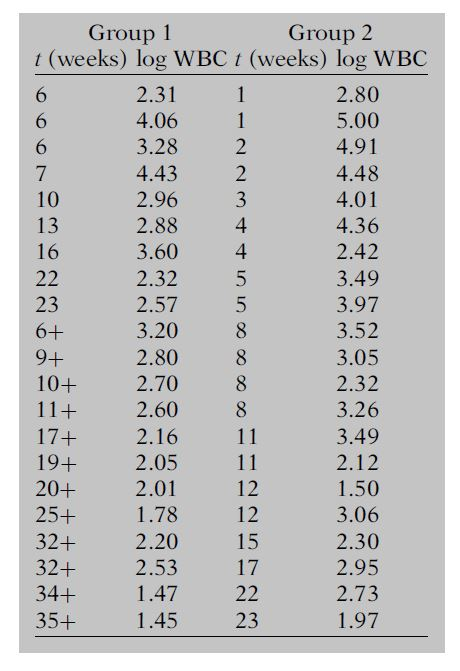
\includegraphics[width =4.5cm, height=5cm]{Ch1-RemissionwLogwbc.JPG}
\end{center}
\end{block}
\end{frame}

\begin{frame}
\frametitle{Variations and Extensions of the Log-Rank Test (cont'd)}
\begin{block}{The stratified log rank test - Remission Data}
We statify on LogWbc with low (1) - 1.45 to 2.30, \\ med (2) - 2.31 to 3.00, high (3) 3.01 to 5.00 and compute:
\begin{columns}
    \begin{column}{0.48\textwidth}
        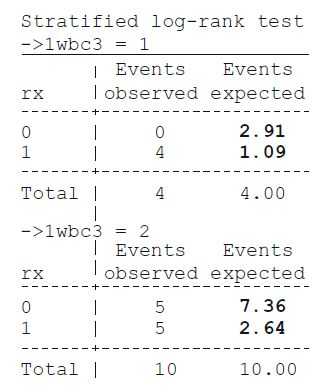
\includegraphics[width =\textwidth, height=5.5cm]{strat_lr1.JPG}
    \end{column}
    \hspace{-10pt}
    \begin{column}{0.48\textwidth}
         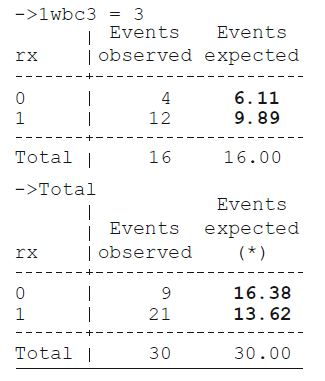
\includegraphics[width =\textwidth, height=5.5cm]{strat_lr2.JPG}
    \end{column}
\end{columns}
\end{block}
\end{frame}

\begin{frame}
\frametitle{Variations and Extensions of the Log-Rank Test (cont'd)}
\begin{block}{Problem 2.5: The stratified log rank test - Remission Data}
\begin{enumerate}
\item Confirm the computations in the previous slide in the first strata (1.50-2.30) of LogWBC.
\item Compute the stratified log rank statistic in R.
\item Make a conclusion about your test and find a $p$-value.
\end{enumerate}
\end{block}
\end{frame}

\begin{frame}
\frametitle{Confidence Intervals about KM estimates}
\begin{block}{Greenwood's formula for SE of estimated survival probabilities}
A 100$(1-\alpha)\%$ CI for the estimated KM survival estimates:
\[
\hat{S}_{KM}(t) \pm z_{\alpha/2}\text{SE}(\hat{S}_{KM}(t))
\]
where $\text{SE}(\hat{S}_{KM}(t)) = \sqrt{Var[\hat{S}_{KM}(t)]}.$
\textbf{By Greenwood's formula}
\[
Var[\hat{S}_{KM}(t)] = (\hat{S}_{KM}(t))^2 \sum_{f:t_{(f)} \le t}\left[\frac{m_f}{n_f(n_f-m_f)}\right]
\]
\end{block}
\end{frame}

\begin{frame}
\frametitle{Confidence Intervals about KM estimates}
\begin{block}{Greenwood's formula for SE of estimated survival probabilities (cont'd)}
\textbf{Greenwood's formula} applied to treatment group in the Remission data
\begin{center}
   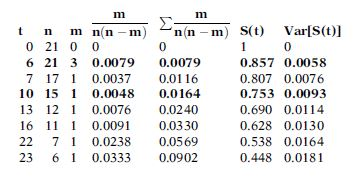
\includegraphics[width =6cm, height=4cm]{Ch2_Greenwoods.JPG}
\end{center}
\end{block}
\end{frame}

\begin{frame}
\frametitle{Confidence Intervals about KM estimates}
\begin{block}{Problem 2.6 - Confidence Intervals for KM estimates}
\begin{enumerate}
\item Find confidence intervals about KM estimates at times 6 and 7 for the treatment group using the above table.
\item Use R to find confidence intervals about the KM estimates for the treatment group.
\item Use R to plot the survival curves and confidence bands for the treatment and placebo groups.
\end{enumerate}
\end{block}
\end{frame}
  %
\begin{frame}
\frametitle{Confidence Interval for the median, $M$}
\begin{block}{Large sample confidence interval for $M$}
We use the large sample distribution
\[ \frac{\hat{S}_{KM}(M) - 0.5}{SE[\hat{S}_{KM}(M)]} \sim Z \text{ where } Z \sim N(0,1) \text { and } M \text{ is the median.}
\]
Thus, we have
\begin{align*}
&P(0.5 - z_{\alpha/2}SE[\hat{S}_{KM}(M)] <  \hat{S}_{KM}(M) < 0.5 + z_{\alpha/2}SE[\hat{S}_{KM}(M)]) \\
&\approx 1-\alpha
\end{align*}
and it is reasonable to take a $1-\alpha$ C.I. for $M$ as all $M$ that satisfy the above inequality. Often, the open interval to the survival times one above the largest $M$'s that satisfies this inequality is used.
\end{block}
\end{frame}


\begin{frame}
\frametitle{Confidence Interval for the median}
\begin{block}{Problem 2.6 - Large sample confidence interval for $M$}
Use R to find a $95\%$ confidence interval for the median for the placebo and survival groups for the Remission data.
\end{block}
\end{frame}

\end{document} 